\section{Server Implementation}

Server was based on NodeJS and was written in JavaScript. It contains implementation of the \hyperref[sec:appendix_a]{OpenAPI definition of RestAPI}. 

Database was set up in external online database server and tools \textit{MongoDB Atlas}. \textit{MongoDB Compass} tool was used to view and modify dataset stored in MongoDB database. Screenshot of the tool is visible at the figure nr \ref{fig:MongoDBCompass}.

\begin{figure}[h]
    \centering
    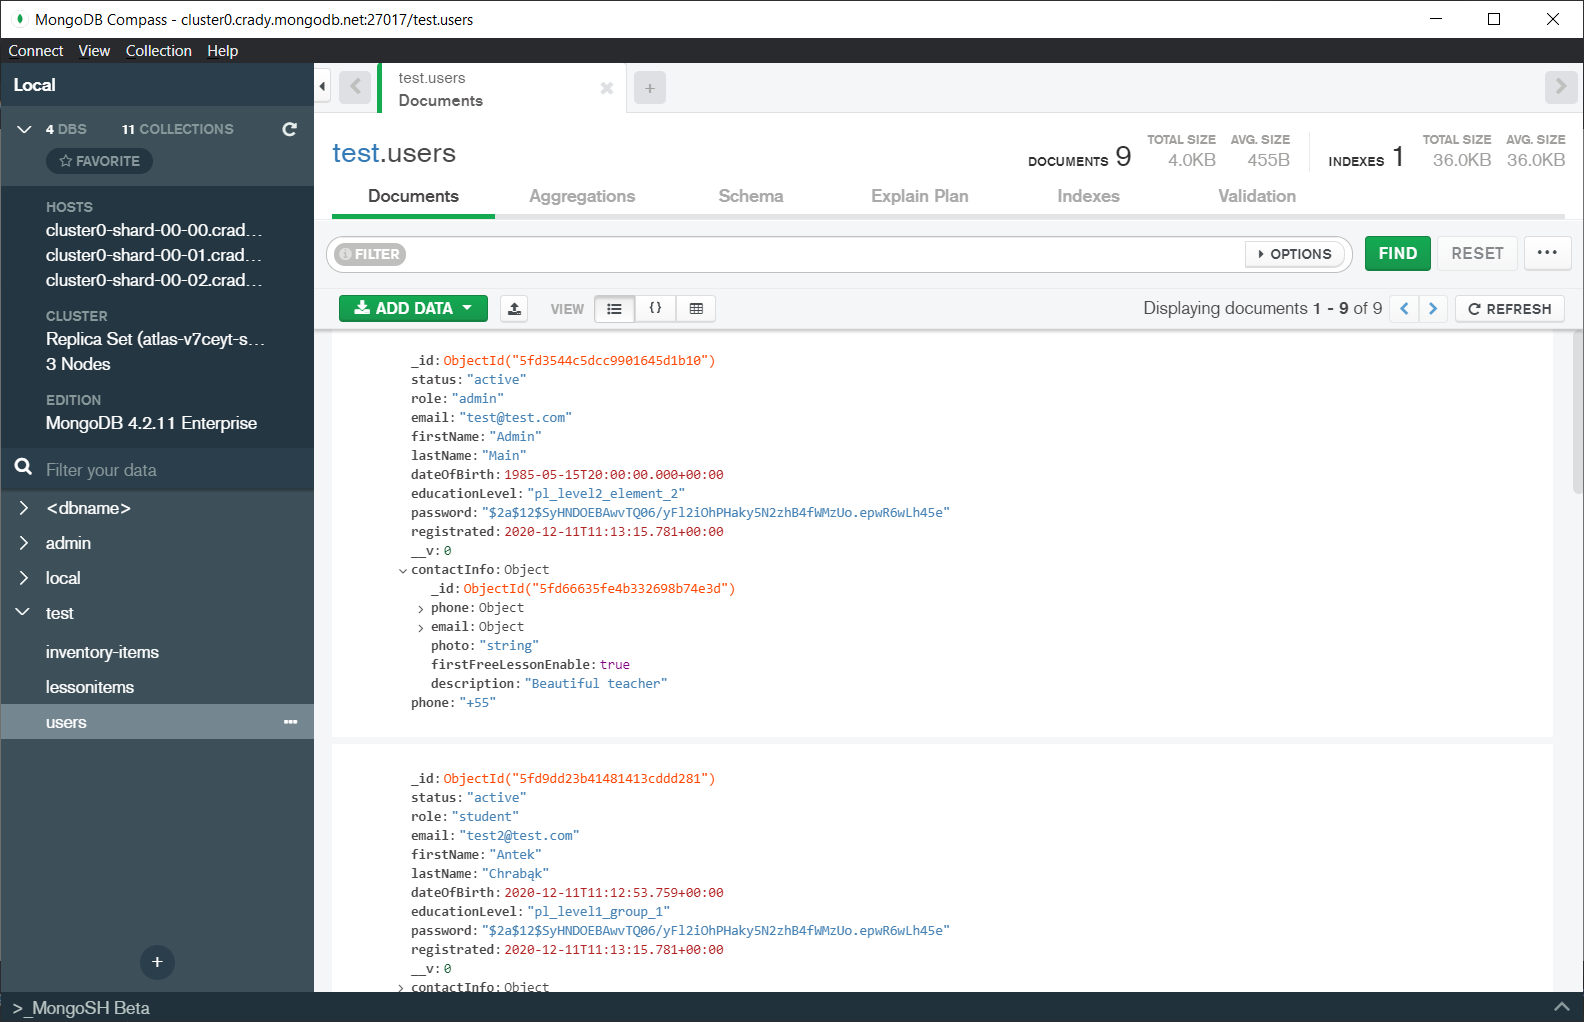
\includegraphics[width=\textwidth]{Include/Resources/MongoDB/MongoDBCompass.png}
    \caption{MongoDB Compass}
    \label{fig:MongoDBCompass}
\end{figure}

To use connect to the MongoDB database import of the mongoose liblary was needed.
\begin{lstlisting}[breaklines=true, numbers=left, stepnumber=1]
const mongoose = require('mongoose');
\end{lstlisting}

To manipulate data in the database mongoose Schema of the collections should be defined. My project contains two collections, so both are defined as separate mongoose Schemas.

Definition of LessonItem object:
\lstinputlisting[breaklines=true, numbers=left, stepnumber=1]{Include/SourceCode/LessonItem.js}

Definition of User object:
\lstinputlisting[breaklines=true, numbers=left, stepnumber=1]{Include/SourceCode/User.js}

In the next step Mongoose Schemas can be imported to server source code:

\begin{lstlisting}[breaklines=true, numbers=left, stepnumber=1]
const User = require('./data/User');
const LessonItem = require('./data/LessonItem');
\end{lstlisting}

One of the most important operations is POST request, that create object in database. Below listing consist operation of adding new lesson item to system.
\begin{lstlisting}[breaklines=true, numbers=left, stepnumber=1]
app.post('/api/v1/lessons', requireAuth, async (req, res) => {
  // operationId: addLessonItem
  errorMessage = 'There was a problem creating your lesson item';
  try {
    const { teacherId,
      educationLevel,
      places,
      teachingLanguages,
      hourlyRate,
      onlineModeEnable,
      faceToFaceModeStudentPlaceEnable,
      faceToFaceModeTeacherPlaceEnable,
      description,
      fieldOfStudy
    } = req.body;

    const lessonsData = {
      teacherId,
      educationLevel,
      places,
      teachingLanguages,
      hourlyRate,
      onlineModeEnable,
      faceToFaceModeStudentPlaceEnable,
      faceToFaceModeTeacherPlaceEnable,
      description,
      fieldOfStudy
    };
    if (req.user.role !== 'admin') {
      lessonsData.teacherId = req.user.id;
    }

    const existingLesson = await LessonItem.findOne({
      teacherId: lessonsData.teacherId,
      fieldOfStudy: lessonsData.fieldOfStudy
    }).lean();

    if (existingLesson) {
      return res
        .status(400)
        .json({ message: 'Lesson already exists' });
    }

    const newLesson = new LessonItem(lessonsData);
    const savedLesson = await newLesson.save();

    if (savedLesson) {
      await updateUserRole(savedLesson.teacherId);
      await updateLessonItemsUserInfoByUserId(savedLesson.teacherId);
      returnLessonItem = await prepareDataLessonItemGet(savedLesson.toObject());
      return res.json(returnLessonItem);
    } else {
      return res.status(400).json({
        message: errorMessage
      });
    }
  } catch (err) {
    console.log(err);
    return res.status(400).json({
      message: errorMessage
    });
  }
});
\end{lstlisting}

GET, PUT and DELETE request can be often takes less lines of code than POST request.
\begin{lstlisting}[breaklines=true, numbers=left, stepnumber=1]
app.get('/api/v1/lessons/:id', async (req, res) => {
    // operationId: getLessonItemId
    try {
        const lessonItem = await LessonItem.findById(req.params.id).lean();
        res.json(lessonItem);
    } catch (err) {
        return res.status(400).json({
        message: 'There was a problem getting the lesson item'
        });
    }
    });
    
    app.put('/api/v1/lessons/:id', requireAuth, async (req, res) => {
    // operationId: updateLessonItemById
    try {
        const lessonItem = await LessonItem.findById(req.params.id).lean();
        if (isUserOwnerOrAdmin(lessonItem.teacherId, req.user.id)) {
        await LessonItem.findOneAndUpdate(
            { _id: req.params.id },
            req.body
        );
        res.json({
            message:
            'Lesson item updated.'
        });
        } else {
        return res.status(401).json({ message: 'Unauthorized' });
        }
    } catch (err) {
        console.log(err);
        return res.status(400).json({
        message: 'There was a problem updating the lesson item'
        });
    }
    });
    
    app.delete('/api/v1/lessons/:id', requireAuth, async (req, res) => {
    // operationId: deleteLessonItemById
    try {
        const lessonItem = await LessonItem.findById(req.params.id).lean();
        if (isUserOwnerOrAdmin(lessonItem.teacherId, req.user.id)) {
        const lessonItem = await LessonItem.findByIdAndRemove(req.params.id);
        await updateUserRole(lessonItem.teacherId);
        res.json({
            message: "Lesson item deleted"
        });
        } else {
        return res.status(401).json({ message: 'Unauthorized' });
        }
    } catch (err) {
        console.log(err);
        return res.status(400).json({
        message: 'There was a problem deleting the lesson item'
        });
    }
    });
\end{lstlisting}

One of the exception can be GET request that is used to find elements with constrains:
\begin{lstlisting}[breaklines=true, numbers=left, stepnumber=1]
app.get('/api/v1/lessons', async (req, res) => {
    // operationId: findLessonItemByStatus
    // firstFreeLesson: req.query.firstFreeLesson
    // availableOnline: true
    searchValue = {};
    
    if (typeof req.query.fieldOfStudy === 'string' || req.query.fieldOfStudy instanceof String) {
        searchValue.fieldOfStudy = req.query.fieldOfStudy;
    }
    
    if (typeof req.query.lessonPlaceMode === 'string' || req.query.lessonPlaceMode instanceof String) {
        searchValue.places = req.query.lessonPlaceMode;
    } else if (req.query.educationLevel instanceof Object) {
        searchValue.places = { $in: req.query.lessonPlaceMode };
    }
    
    if (typeof req.query.educationLevel === 'string' || req.query.educationLevel instanceof String) {
        searchValue.educationLevel = req.query.educationLevel;
    } else if (req.query.educationLevel instanceof Object) {
        searchValue.educationLevel = { $in: req.query.educationLevel };
    }
    
    if (typeof req.query.teachingLanguages === 'string' || req.query.teachingLanguages instanceof String) {
        searchValue.teachingLanguages = req.query.teachingLanguages;
    } else if (req.query.teachingLanguages instanceof Object) {
        searchValue.teachingLanguages = { $in: req.query.teachingLanguages };
    }
    
    if (req.query.hourlyRateMin !== undefined && req.query.hourlyRateMax !== undefined) {
        searchValue.hourlyRate = { $gte: req.query.hourlyRateMin, $lte: req.query.hourlyRateMax };
    } else if (req.query.hourlyRateMin !== undefined) {
        searchValue.hourlyRate = { $gte: req.query.hourlyRateMin };
    } else if (req.query.hourlyRateMax !== undefined) {
        searchValue.hourlyRate = { $lte: req.query.hourlyRateMax };
    }
    
    // console.log(searchValue);
    
    try {
        const lessonItems = await LessonItem.find(searchValue).lean();
        res.json(lessonItems);
    } catch (err) {
        console.log(err);
        return res.status(400).json({
        message: 'There was a problem getting the lesson item'
        });
    }
    });      
\end{lstlisting}

Example data of users exported from database. First object is student user:
\begin{lstlisting}[breaklines=true, numbers=left, stepnumber=1]
{
   "_id":{
      "$oid":"5fd9dd23b41481413cddd281"
   },
   "status":"active",
   "role":"student",
   "email":"test2@test.com",
   "firstName":"Antek",
   "lastName":"Chrabak",
   "dateOfBirth":{
      "$date":"2020-12-11T11:12:53.759Z"
   },
   "educationLevel":"pl_level1_group_1",
   "password":"$2a$12$SyHNDOEBAwvTQ06/yFl2iOhPHaky5N2zhB4fWMzUo.epwR6wLh45e",
   "registrated":{
      "$date":"2020-12-11T11:13:15.781Z"
   },
   "__v":0,
   "contactInfo":{
      "_id":{
         "$oid":"5ff1a3c854ce411748ee12a4"
      },
      "phone":{
         "_id":{
            "$oid":"5ff1a3c854ce411748ee12a5"
         },
         "number":"111111111",
         "visible":true
      },
      "email":{
         "_id":{
            "$oid":"5ff1a3c854ce411748ee12a6"
         },
         "email":"1111@aa",
         "visible":true
      },
      "firstFreeLessonEnable":true,
      "description":"Beautiful teacher"
   }
}
\end{lstlisting}

Second example is teacher user:
\begin{lstlisting}[breaklines=true, numbers=left, stepnumber=1]
    {
   "_id":{
      "$oid":"5fdbd2f59b290b21e80697c9"
   },
   "status":"active",
   "role":"teacher",
   "email":"test3@test.com",
   "firstName":"Antoni",
   "lastName":"Andrzejek",
   "dateOfBirth":{
      "$date":"2018-12-12T22:00:00.000Z"
   },
   "educationLevel":"pl_level3_element_1",
   "password":"$2a$12$7.xqpqVsqsFRH6KWlfOYueN5OSbR/WlMAY8.fBZk.eMFnCWIyVVgu",
   "registrated":{
      "$date":"2020-12-11T11:13:15.781Z"
   },
   "__v":0,
   "phone":"+46111",
   "contactInfo":{
      "_id":{
         "$oid":"5ff1fe63116c8417700a140d"
      },
      "phone":{
         "_id":{
            "$oid":"5ff1fe63116c8417700a140e"
         },
         "number":"+118000",
         "visible":true
      },
      "email":{
         "_id":{
            "$oid":"5ff1fe63116c8417700a140f"
         },
         "email":"niepiszdomnie@cc.ok",
         "visible":true
      },
      "firstFreeLessonEnable":true,
      "description":"Lorem Ipsum is simply dummy text of the printing and typesetting industry. Lorem Ipsum has been the industry's standard dummy text ever since the 1500s, when an unknown printer took a galley of type and scrambled it to make a type specimen book. It has survived not only five centuries, but also the leap into electronic typesetting, remaining essentially unchanged. It was popularised in the 1960s with the release of Letraset sheets containing Lorem Ipsum passages, and more recently with desktop publishing software like Aldus PageMaker including versions of Lorem Ipsum."
   }
}
\end{lstlisting}

Example below presents Lesson Item object stored in database:
\begin{lstlisting}[breaklines=true, numbers=left, stepnumber=1]
{
    "_id":{
        "$oid":"5fef6ce79a838e2e9823f02f"
    },
    "educationLevel":[
        "pl_level3_element_1"
    ],
    "places":[
        
    ],
    "teachingLanguages":[
        "teach_lan_spanish"
    ],
    "teacherId":{
        "$oid":"5fdbd2f59b290b21e80697c9"
    },
    "hourlyRate":0,
    "onlineModeEnable":true,
    "faceToFaceModeStudentPlaceEnable":true,
    "faceToFaceModeTeacherPlaceEnable":true,
    "description":"asdasdasd",
    "fieldOfStudy":"lan_french",
    "lessonFeedback":[
        {
            "valuableFeedback":[
                
            ],
            "notValuableFeedback":[
                
            ],
            "_id":{
                "$oid":"5ff2266e3b7b0c3fac6cf922"
            },
            "description":"lkajsdlkamdlsk",
            "rating":3,
            "studentId":{
                "$oid":"5ff224fc68be3343182fe527"
            },
            "feedbackPostDate":{
                "$date":"2021-01-03T20:17:50.725Z"
            }
        }
    ],
    "__v":0,
    "email":"niepiszdomnie@cc.ok",
    "firstFreeLessonEnable":true,
    "phoneNumber":"+118000",
    "numberOfFeedbacks":1,
    "rating":3
}
\end{lstlisting}

% \begin{lstlisting}[breaklines=true, numbers=left, stepnumber=1]
% \end{lstlisting}